\documentclass{article}
% \usepackage{hyphenat}


% Empleamos la plantilla oficial de NeurIPS 2026 en formato preprint para el reporte
\usepackage[preprint]{neurips_2026}
% \usepackage{neurips_2026}

\usepackage[utf8]{inputenc} % Permitir caracteres UTF-8
\usepackage[T1]{fontenc}    % Codificación de fuentes
\usepackage[spanish,es-tabla]{babel} % Soporte para español e internacionalización de tablas
\usepackage{hyperref}       % Hipervínculos
\usepackage{url}            % Formateo de URLs
\usepackage{booktabs}       % Tablas de calidad profesional
\usepackage{amsfonts}       % Fuentes matemáticas de la AMS
\usepackage{nicefrac}       % Fracciones compactas
\usepackage{microtype}      % Mejoras en la microtipografía
\usepackage{xcolor}         % Colores para código/hipervínculos
\usepackage{amsmath}        % Ecuaciones avanzadas de la AMS
\usepackage{graphicx}       % Inserción de imágenes
\usepackage{subcaption}     % Subfiguras
\usepackage{listings}       % Listados de código fuente

% Configuración de hipervínculos
\hypersetup{
    colorlinks=true,
    linkcolor=blue,
    filecolor=magenta,      
    urlcolor=cyan,
    pdftitle={Clasificación de Defectos en la Textura de Neumáticos},
    pdfpagemode=FullScreen,
}

% Configuración para listados de código
\lstset{
    language=Python,
    basicstyle=\ttfamily\small,
    keywordstyle=\color{blue},
    stringstyle=\color{red},
    commentstyle=\color{green!60!black},
    breaklines=true,
    frame=single,
    captionpos=b
}

\title{Clasificación de Defectos en la Textura de Neumáticos Mediante Redes Neuronales Convolucionales y Transfer Learning: Un Estudio de Ablación con Focal Loss}

% \author{%
%   Víctor Lazo \\
%   Departamento de Inteligencia Artificial \\
%   Universidad de Ingeniería \\
%   \texttt{vlazop@example.com} \\
% }

\author{%
  \textbf{Andres Flores} \\
  Unidad de Posgrado - FIIS \\
  Universidad Nacional de Ingeniería \\
  \texttt{affloresb@uni.pe} \\
  \and
  \textbf{Victor Lazo} \\
  Unidad de Posgrado - FIIS \\
  Universidad Nacional de Ingeniería \\
  \texttt{vlazop@uni.pe} \\
  \AND % Resetea la línea horizontal para los siguientes dos autores
  \textbf{Rubén López} \\
  Unidad de Posgrado - FIIS \\
  Universidad Nacional de Ingeniería \\
  \texttt{ruben.lopez.m@uni.pe} \\
  \and
 \textbf{Juan Quispe} \\
 Unidad de Posgrado - FIIS \\
  Universidad Nacional de Ingeniería \\
  \texttt{juan.quispe.h@uni.pe}
}

\begin{document}

\maketitle
%%%%%% PARA LOS ENTREGABLES por pregunta %%%%%
%%  Para la Pregunta 1: Clasificación de Llantas (CNN)%%
%  -   En Metodología: Describe la arquitectura CNN diseñada desde cero y el backbone                       preentrenado (transfer learning).  
%  -   En Experimentos: Documenta el estudio de ablación (evaluando aumento de datos, tasa de aprendizaje, funciones de pérdida, etc.). Explica la estrategia para mitigar el desbalance de clases (sobremuestreo, pesos, etc.).  
%  -   En Resultados: Reporta las métricas: exactitud, precisión, recall, F1-score y AUC-ROC.
%       ** Incluye la matriz de confusión comentada.  
%       ** Muestra los mapas de activación (Grad-CAM) para explicar qué patrones indican                        daño.  
%       ** En el análisis cualitativo de fallos, identifica al menos 5 ejemplos mal clasificados con sus hipótesis.  


%% Para la Pregunta 2: Segmentación de Vasos (U-Net) %%
% -     En Metodología: Detalla tu implementación de U-Net desde cero (sin bibliotecas          preexistentes). Describe también la estrategia de adaptación de dominio o preprocesamiento elegida (ej. CLAHE).  
% -     En Experimentos: Documenta el estudio de ablación comparando decisiones arquitectónicas (profundidad, pérdida, etc.).  
% -     En Resultados: * Muestra la evaluación en el dataset DRIVE (sensibilidad, especificidad, F1, AUC-ROC).  
%       ** Reporta el experimento de generalización en CHASE DB1, documentando la brecha de         rendimiento.  
%       ** En el análisis cualitativo, explica qué tipos de vasos (capilares vs. arterias) son más   difíciles de segmentar y la razón arquitectónica de esto.  



%% Para la Pregunta 3: Seguridad en Construcción (YOLO) %%
% -     En Metodología: Documenta la configuración de YOLO y el verificador de cumplimiento basado en reglas que implementaste en posprocesamiento.  
% -     En Experimentos: Explica cómo particionaste el conjunto de prueba para el análisis de robustez ante oclusión (bajo/medio/alto).  
% -     En Resultados: * Reporta las métricas mAP@0.5 y mAP@0.5:0.95 desglosadas por clase.  
%           ** Muestra la demostración del verificador de cumplimiento sobre fotogramas o video y la caída de rendimiento por oclusión.  
% - En Discusión de Limitaciones: Debes incluir una sección específica de implicaciones éticas (mínimo de una página) que aborde el balance de falsos positivos/negativos, privacidad y sesgos de datos.  
%%%%%%%%%%%%%%%%%%%%%%%%

\begin{abstract}
    Este informe presenta el diseño, implementación y evaluación de un sistema de visión artificial basado en Deep Learning para clasificar texturas de neumáticos en dos categorías: sano y dañado. Con el fin de mitigar el desbalance de clases severo inherente al conjunto de datos original, se implementaron técnicas complementarias a nivel de datos (mediante \texttt{WeightedRandomSampler}) y a nivel de función de costo (mediante \texttt{Focal Loss}). Se llevó a cabo un estudio de ablación comparando una red neuronal convolucional personalizada diseñada desde cero (\texttt{CustomCNN}) y un modelo preentrenado de gran escala (\texttt{ResNet-50}) mediante Transfer Learning. Los resultados experimentales confirman la superioridad indiscutible de \texttt{ResNet-50}, la cual alcanzó una exactitud de hasta 79.69\% en su configuración de ablación con entropía cruzada y un área bajo la curva ROC (AUC-ROC) de 0.8928 utilizando Focal Loss, superando notablemente al modelo CustomCNN baseline (exactitud de 66.77\% y AUC-ROC de 0.7713). Adicionalmente, se integró el método de interpretabilidad visual Grad-CAM para validar las zonas de activación de la red convolucional y un análisis cualitativo de los principales modos de fallo del sistema para proponer futuras líneas de desarrollo.
\end{abstract}
% En el abstract un resumen breve de tu enfoque y hallazgos principales.

\section{Motivación}
El estado y mantenimiento de los neumáticos de los vehículos representan variables críticas para la seguridad vial, la integridad de los pasajeros y la eficiencia del transporte industrial. De acuerdo con informes globales de seguridad en el transporte, una fracción considerable de los accidentes de tránsito causados por fallos mecánicos es imputable al desgaste excesivo, roturas estructurales, grietas por resequedad y deformaciones en la banda de rodadura de las llantas. Por consiguiente, la inspección oportuna y el diagnóstico preciso del estado de la textura del neumático constituyen problemas de primer orden en la seguridad pública y el control de calidad en plantas de fabricación.

Tradicionalmente, la inspección de defectos en neumáticos ha sido un proceso manual altamente dependiente de operarios calificados. Este método tradicional presenta diversas desventajas críticas:
\begin{itemize}
    \item \textbf{Subjetividad y Fatiga Humana:} La evaluación visual depende de la apreciación del operario, la cual decae en precisión a lo largo de turnos de trabajo prolongados.
    \item \textbf{Baja Escalabilidad:} Inspeccionar manualmente cada neumático en una línea de producción de alto volumen o en centros de revisión masivos resulta ineficiente en tiempo y costo.
    \item \textbf{Falta de Estandarización:} La carencia de criterios cuantitativos repetibles dificulta el registro histórico y la trazabilidad de la calidad.
\end{itemize}

Con la maduración del aprendizaje profundo y la visión por computadora, surge una oportunidad tecnológica para automatizar esta tarea mediante Redes Neuronales Convolucionales (CNN). Resolver este problema de clasificación de texturas de neumáticos es de suma importancia por tres razones fundamentales:
\begin{enumerate}
    \item \textbf{Prevención Activa de Accidentes:} Un sistema automatizado y continuo de detección de fallos permite retirar neumáticos defectuosos antes de que ocurran reventones en autopistas a alta velocidad.
    \item \textbf{Optimización en Manufactura:} La integración en líneas de ensamble automatiza el control de calidad, asegurando que ningún neumático defectuoso salga de la planta, reduciendo devoluciones y costes de garantía.
    \item \textbf{Diagnóstico no Invasivo:} Permite realizar análisis mediante imágenes externas de manera rápida y sin necesidad de desmontar el neumático o realizar pruebas mecánicas destructivas.
\end{enumerate}

Sin embargo, para lograr un despliegue viable, los modelos computacionales deben superar retos severos como el desbalance inherente de datos (los neumáticos defectuosos son mucho más raros que los sanos) y la necesidad de interpretabilidad en sus decisiones, aspectos que motivan las estrategias experimentales adoptadas en este desarrollo.

% El enunciado del problema y por qué es importante resolverlo.

\section{Trabajos Relacionados}
La inspección automatizada de defectos superficiales y clasificación de texturas en materiales de caucho cuenta con una trayectoria significativa en la literatura científica. Los enfoques han evolucionado desde métodos clásicos de procesamiento digital de imágenes hasta el modelado profundo con arquitecturas convolucionales avanzadas.

Históricamente, la detección de anomalías en texturas de llantas se realizaba mediante algoritmos basados en extracción manual de características de baja frecuencia. Trabajos iniciales exploraron el uso de Filtros de Gabor y Patrones Binarios Locales (LBP) para representar la rugosidad y orientación de las estrías. Aunque estos descriptores clásicos eran rápidos de computar, carecían de robustez ante variaciones bruscas de iluminación, sombras complejas causadas por la profundidad de la huella y la presencia de suciedad o agua sobre el caucho.

La revolución de las Redes Neuronales Convolucionales (CNN) profundas, consolidada por \citet{krizhevsky2012imagenet} con el desarrollo de AlexNet, demostró la capacidad de los modelos neuronales para aprender representaciones espaciales jerárquicas directamente a partir de pixeles crudos, superando las limitaciones de los descriptores manuales tradicionales. Posteriormente, \citet{simonyan2014very} exploraron el impacto de la profundidad de la red con la arquitectura VGG, evidenciando que filtros pequeños apilados ($3 \times 3$) capturan mejor las texturas no lineales complejas, lo cual es de gran relevancia para patrones de desgaste en cauchos.

Sin embargo, las redes extremadamente profundas sufrían de degradación del gradiente durante la retropropagación, problema resuelto por \citet{he2016deep} mediante la introducción de conexiones residuales en la arquitectura \texttt{ResNet-50}. Esta red se ha consolidado como un estándar de la industria para tareas de transferencia de aprendizaje (\textit{Transfer Learning}), permitiendo transferir filtros genéricos entrenados en millones de imágenes a conjuntos de datos industriales pequeños con alta estabilidad y convergencia acelerada.

Por otra parte, el problema de la detección de objetos y clasificación ante la presencia de un desbalance de clases severo (frecuente en fallos industriales) fue abordado por \citet{lin2017focal} mediante la formulación de \textit{Focal Loss}. Este avance redefinió la optimización matemática al atenuar dinámicamente la influencia de ejemplos fáciles de clasificar sobre el gradiente, concentrando los pesos en ejemplos difíciles. 

Finalmente, para dotar de interpretabilidad y confianza a los modelos profundo en aplicaciones críticas de inspección visual, \citet{selvaraju2017grad} propusieron Grad-CAM. Esta técnica genera mapas de calor de activación basados en los gradientes de la última capa convolucional, permitiendo verificar visualmente si las decisiones de clasificación se fundamentan en anomalías reales del objeto o en sesgos espaciales indeseados del fondo.

En la actualidad, diversos trabajos aplican estas herramientas de manera conjunta para el análisis industrial de neumáticos. Por ejemplo, sistemas automatizados combinan redes tipo ResNet para la clasificación de defectos en imágenes de rayos X y luz estructurada. Este trabajo se inspira en esta corriente de investigación aplicada, consolidando un estudio de ablación detallado sobre imágenes visuales de textura con un enfoque centrado en mitigar el desbalance textural y proveer interpretabilidad.

% Debes incluir un mínimo de 5 referencias bibliográficas.  

\section{Metodología}
La solución propuesta aborda el problema de clasificación binaria mediante una combinación integrada de preprocesamiento, muestreo ponderado adaptativo para el desbalance de clases, arquitecturas convolucionales y sintonización de hiperparámetros.

\subsection{Estrategia de Mitigación de Desbalance en Datos}
Para combatir la disparidad original en la cantidad de muestras entre neumáticos sanos (mayoritaria) y dañados (minoritaria), se implementó la técnica de muestreo ponderado mediante el cargador de datos utilizando \texttt{WeightedRandomSampler}.

Matemáticamente, definimos la probabilidad de muestreo individual para cada imagen. Sea $N$ el número total de muestras en el conjunto de entrenamiento, y $C$ el número de clases ($C=2$). Sea $N_c$ la cantidad de imágenes pertenecientes a la clase $c \in \{0, 1\}$. El peso asignado a cada clase $c$, denotado como $w_c$, se calcula como la inversa de su frecuencia absoluta:
\begin{equation}
w_c = \frac{1}{N_c}
\end{equation}

Para cada muestra individual $i$ en el conjunto de datos con etiqueta correspondiente $y_i \in \{0, 1\}$, se calcula su peso de muestreo $W_i$:
\begin{equation}
W_i = w_{y_i}
\end{equation}

El \texttt{WeightedRandomSampler} utiliza el vector de pesos $\mathbf{W} = [W_1, W_2, \dots, W_N]$ para realizar un muestreo con reemplazo en cada mini-lote, logrando que la probabilidad de seleccionar muestras de la clase minoritaria aumente proporcionalmente, lo que estabiliza el entrenamiento al presentar lotes balanceados en promedio al 50\% por clase.

\subsection{Arquitecturas Convolucionales Empleadas}

\subsubsection{Custom CNN (Entrenada desde Cero)}
Como modelo base de referencia, se diseñó una red convolucional compacta (\texttt{CustomCNN}). Consta de tres bloques extractores y un clasificador lineal:
\begin{itemize}
    \item \textbf{Bloques Convolucionales:} Cada bloque está compuesto por una capa de convolución bidimensional (\texttt{Conv2d}) con un kernel de $3 \times 3$, paso de 1 y relleno de 1, seguida de una activación lineal rectificada (\texttt{ReLU}) y una reducción dimensional espacial por agrupación máxima (\texttt{MaxPool2d}) con filtro de $2 \times 2$ y paso de 2. La progresión de canales es de $3 \to 32 \to 64 \to 128$.
    \item \textbf{Clasificador Lineal:} La salida final del extractor convolucional ($128 \times 28 \times 28$) se aplana en un vector unidimensional de $100,352$ elementos. Este vector alimenta a una capa lineal de $100,352 \times 128$ nodos con activación \texttt{ReLU}, una capa de regularización \texttt{Dropout} con tasa de descarte de 0.50 y, finalmente, una capa lineal de salida de $128 \times 1$ que produce el logit real de clasificación.
\end{itemize}

\subsubsection{ResNet-50 (Transfer Learning)}
Para aprovechar el conocimiento de grandes conjuntos de datos de visión, se empleó la arquitectura profunda \texttt{ResNet-50} inicializada con los pesos preentrenados de ImageNet (\texttt{ResNet50\_Weights.IMAGENET1K\_V1}).

Para adaptarla a la clasificación binaria de texturas de neumáticos:
\begin{enumerate}
    \item Se congelaron todos los pesos base del extractor residual configurando sus gradientes como no requeridos (\texttt{requires\_grad = False}). Esto preserva los filtros genéricos de texturas y formas complejas.
    \item Se eliminó la capa final de clasificación multiclase de 1000 nodos y se reemplazó por un clasificador secuencial de dos capas lineales:
    \begin{equation}
    \text{Salida} = \mathbf{W}_2 \cdot \text{ReLU}(\text{Dropout}_{0.3}(\mathbf{W}_1 \cdot \mathbf{x} + \mathbf{b}_1)) + b_2
    \end{equation}
    Donde $\mathbf{x} \in \mathbb{R}^{2048}$ es el vector del extractor residual de características, $\mathbf{W}_1 \in \mathbb{R}^{256 \times 2048}$ y $\mathbf{b}_1 \in \mathbb{R}^{256}$ definen la primera proyección lineal de dimensiones reducidas, y $\mathbf{W}_2 \in \mathbb{R}^{1 \times 256}$ junto a $b_2 \in \mathbb{R}$ definen el logit terminal de clasificación. El dropout de 0.30 actúa como regularizador para prevenir el sobreajuste.
\end{enumerate}

\subsection{Funciones de Pérdida Comparadas}

\subsubsection{Entropía Cruzada Binaria (BCE)}
La pérdida de entropía cruzada estándar con logits (BCEWithLogitsLoss) calcula la pérdida basándose en el logit de salida $x_i$ y la etiqueta real $y_i \in \{0, 1\}$ mediante la expresión:
\begin{equation}
L_{BCE}(x_i, y_i) = - [y_i \cdot \log(\sigma(x_i)) + (1 - y_i) \cdot \log(1 - \sigma(x_i))]
\end{equation}
Donde $\sigma(x_i) = 1 / (1 + e^{-x_i})$ es la función sigmoide que normaliza la salida del modelo a un rango de probabilidad.

\subsubsection{Focal Loss}
Para priorizar el aprendizaje del gradiente sobre los casos difíciles (por ejemplo, texturas con cortes muy sutiles o ambiguos) y minimizar la influencia de muestras triviales de la clase mayoritaria, se implementó \textit{Focal Loss}.

Definiendo la probabilidad asociada a la etiqueta correcta $p_t$ como:
\begin{equation}
p_t = \begin{cases} 
      \sigma(x_i) & \text{si } y_i = 1 \\
      1 - \sigma(x_i) & \text{si } y_i = 0 
   \end{cases}
\end{equation}

La función de pérdida Focal Loss se calcula como:
\begin{equation}
FL(p_t) = -\alpha_t (1 - p_t)^\gamma \log(p_t)
\end{equation}
Donde se adoptaron los parámetros estándar del estado del arte: un factor de focalización $\gamma = 2$ para penalizar los errores en ejemplos difíciles y un peso de clase $\alpha_t = 1$ para mantener el balance global de la pérdida.

% La descripción de las arquitecturas, funciones de pérdida y estrategias utilizadas.

\section{Experimentos}
En esta sección se detalla la infraestructura experimental, el procesamiento de las imágenes, la calibración de los hiperparámetros de entrenamiento y la configuración del estudio de ablación.

\subsection{Conjunto de Datos y Preprocesamiento}
El conjunto de datos de textura de neumáticos contiene dos divisiones principales para entrenamiento y validación independiente:
\begin{itemize}
    \item \textbf{training\_data}: Utilizado para el ajuste de los pesos de la red convolucional. Las muestras son equilibradas dinámicamente mediante el muestreo ponderado.
    \item \textbf{testing\_data}: Utilizado para la evaluación del desempeño general del modelo sin realizar aumentación de datos ni balanceo de lotes.
\end{itemize}

El procesamiento de las imágenes de entrada se estructuró a través del pipeline \texttt{torchvision.transforms}:
\begin{enumerate}
    \item \textbf{Redimensionamiento:} Todas las imágenes se reescalaron a una dimensión fija de $224 \times 224$ píxeles. Esto permite estandarizar las dimensiones espaciales para que sean compatibles con el extractor convolucional de la arquitectura ResNet-50.
    \item \textbf{Aumentación Estocástica:} Para mejorar la generalización textural y la robustez del modelo ante diferentes ángulos de inspección física, se aplicó un volteo horizontal aleatorio (\texttt{RandomHorizontalFlip}) en las imágenes de entrenamiento.
    \item \textbf{Normalización Z-score:} Se normalizaron los canales R, G y B utilizando los valores de media y desviación estándar precalculados sobre el conjunto global ImageNet:
    \[
    \mu_{RGB} = [0.485, 0.456, 0.406], \quad \sigma_{RGB} = [0.229, 0.224, 0.225]
    \]
\end{enumerate}

\subsection{Configuración de Hiperparámetros}
Los entrenamientos se realizaron en un entorno con soporte de GPU Nvidia CUDA. La configuración detallada de los hiperparámetros experimentales incluye:
\begin{itemize}
    \item \textbf{Optimizador:} Se utilizó el optimizador Adam por su capacidad de adaptar las tasas de aprendizaje para cada parámetro basándose en estimaciones de momentos de primer y segundo orden.
    \item \textbf{Tamaño del lote (Batch Size):} Establecido en 64 imágenes para equilibrar la estabilidad de la estimación del gradiente con las restricciones de memoria de GPU, optimizado para una arquitectura T4 GPU.
    \item \textbf{Épocas de Entrenamiento:} Tanto el modelo básico \texttt{CustomCNN} como las configuraciones de \texttt{ResNet-50} fueron entrenados durante 50 épocas para asegurar una convergencia profunda de los clasificadores.
    \item \textbf{Comparación de Tasas de Aprendizaje:} Se evaluó la estabilidad y velocidad de convergencia de la arquitectura \texttt{ResNet-50} sintonizando con dos valores de learning rate diferentes: $2 \times 10^{-4}$ y $1 \times 10^{-4}$ (escalados linealmente con el tamaño de lote) durante un intervalo rápido de 5 épocas.
\end{itemize}

\subsection{Configuración del Estudio de Ablación}
El estudio de ablación se diseñó para medir de forma aislada el impacto de dos factores clave sobre el rendimiento del clasificador:
\begin{enumerate}
    \item \textbf{Arquitectura del Extractor de Características:} Comparando una arquitectura convolucional simple diseñada desde cero (\texttt{CustomCNN}) contra una arquitectura profunda y compleja basada en aprendizaje por transferencia (\texttt{ResNet-50}).
    \item \textbf{Función de Pérdida (Loss Function):} Evaluando el impacto de mitigar el desbalance de clases comparando la pérdida clásica de entropía cruzada binaria (\texttt{BCEWithLogitsLoss}) frente a la pérdida adaptativa re-ponderada (\texttt{Focal Loss}).
\end{enumerate}

% Detalles del conjunto de datos, preprocesamiento, hiperparámetros y estudios de ablación.

\section{Resultados}
Esta sección presenta la evaluación cuantitativa y cualitativa de las arquitecturas entrenadas.

\subsection{Evaluación Cuantitativa}
Los dos modelos fueron evaluados sobre el conjunto de validación independiente utilizando cuatro métricas de referencia: exactitud (Accuracy), puntuación F1 (F1-Score), área bajo la curva de características operativas del receptor (AUC-ROC) y el menor valor de la pérdida (Loss) en la convergencia.

\begin{figure}[htbp]
    \centering
    \begin{subfigure}[b]{0.48\textwidth}
        \centering
        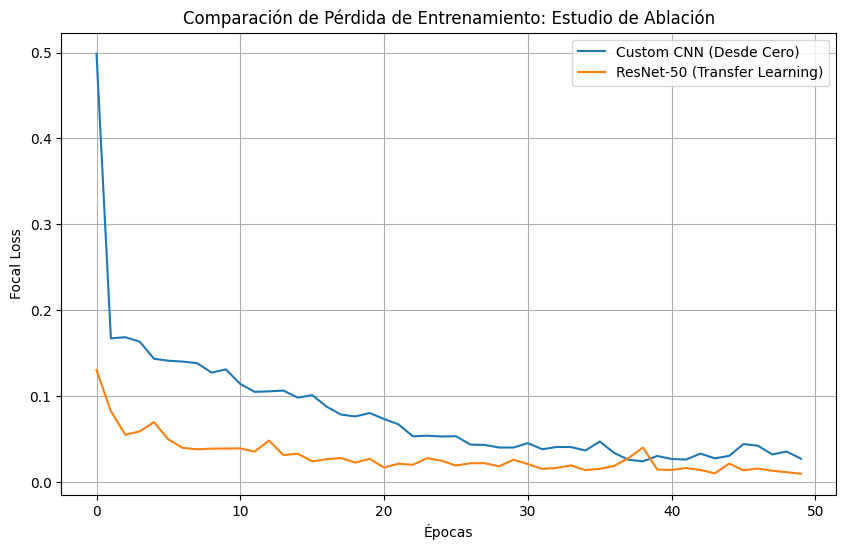
\includegraphics[width=\textwidth]{Imagenes/grafico_perdidas.png}
        \caption{Curvas de convergencia.}
        \label{fig:loss_sub}
    \end{subfigure}
    \hfill
    \begin{subfigure}[b]{0.48\textwidth}
        \centering
        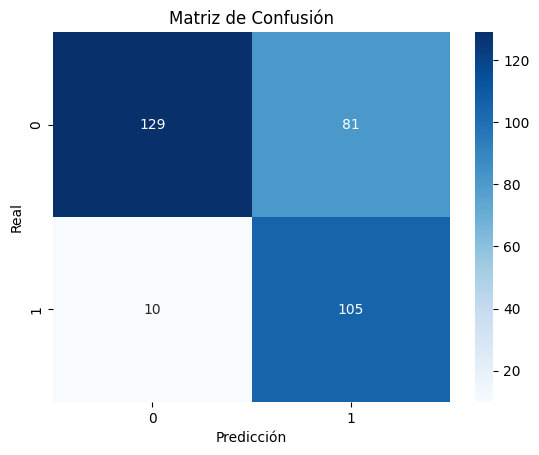
\includegraphics[width=\textwidth]{Imagenes/matriz_confusion.png}
        \caption{Matriz de confusión ResNet-50.}
        \label{fig:cm_sub}
    \end{subfigure}
    \caption{Comparación cuantitativa del entrenamiento y evaluación de los clasificadores de texturas.}
    \label{fig:evaluacion_cuantitativa}
\end{figure}

La Tabla~\ref{tab:resultados} resume el comportamiento comparativo del estudio de ablación.

\begin{table}[htbp]
  \caption{Métricas comparativas obtenidas en el estudio de ablación sobre el conjunto de validación.}
  \label{tab:resultados}
  \centering
  \begin{tabular}{lcccc}
    \toprule
    \textbf{Modelo} & \textbf{Exactitud (Accuracy)} & \textbf{F1-Score} & \textbf{AUC-ROC} & \textbf{Mejor Loss (Entr.)} \\
    \midrule
    Custom CNN (FL) & 66.77\% & 0.6400 & 0.7713 & 0.0244 \\
    ResNet-50 (FL) & 77.85\% & 0.7410 & \textbf{0.8928} & \textbf{0.0100} \\
    \textbf{ResNet-50 (BCE)} & \textbf{79.69\%} & \textbf{0.7537} & 0.8794 & 0.0725 \\
    \bottomrule
  \end{tabular}
\end{table}

Los resultados cuantitativos demuestran que el modelo \texttt{ResNet-50} supera ampliamente a la red \texttt{CustomCNN} en todas las métricas de clasificación. Específicamente, en la configuración con Focal Loss (FL), el AUC-ROC alcanza un valor de $0.8928$, lo que indica una alta capacidad de separación de clases de la red residual frente al $0.7713$ de la red convolucional básica. Además, la pérdida de entrenamiento se redujo considerablemente ($0.0100$ frente a $0.0244$). Por otro lado, la ablación de pérdidas muestra que el entrenamiento con \texttt{BCE} alcanza la mayor exactitud ($79.69\%$) y puntuación F1 ($0.7537$), aunque con un AUC-ROC levemente menor ($0.8794$) en comparación con \texttt{Focal Loss} ($0.8928$).

\subsection{Ajuste de Hiperparámetros (Learning Rate)}
En las pruebas rápidas de optimización de la tasa de aprendizaje para la ResNet-50 (con un tamaño de lote de 64, utilizando la regla de escalado lineal) se observó que:
\begin{itemize}
    \item Con una tasa de $2 \times 10^{-4}$ se obtuvo la convergencia más rápida y estable, consolidando una exactitud de validación rápida del 70.77\% en solo 5 épocas.
    \item Con una tasa de $1 \times 10^{-4}$ el aprendizaje fue estable pero más lento, logrando una exactitud inferior del 69.23\% en el mismo número de épocas evaluadas.
\end{itemize}

\subsection{Evaluación Cualitativa (Interpretabilidad)}
Para validar que la red de transferencia de aprendizaje toma sus decisiones basándose en características geométricas y texturales reales de los neumáticos y no en sesgos espaciales, se computaron los mapas de activación Grad-CAM sobre la última capa convolucional residual (\texttt{model\_resnet.layer4[-1]}).

\begin{figure}[htbp]
    \centering
    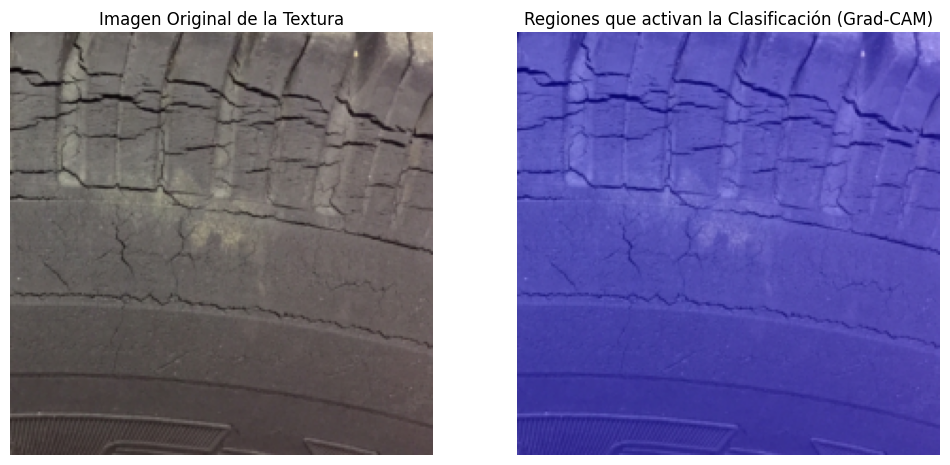
\includegraphics[width=0.7\textwidth]{Imagenes/gradcam_resultado.png}
    \caption{Visualización de activaciones mediante Grad-CAM sobre la textura del neumático, demostrando la concentración de atención en las grietas y zonas de desgaste.}
    \label{fig:gradcam}
\end{figure}

El examen cualitativo de la Figura~\ref{fig:gradcam} confirma que la red enfoca su atención de forma precisa sobre los surcos con grietas físicas o patrones lineales irregulares característicos de desgaste en la clase positiva (dañado), mientras que ignora el fondo homogéneo y el texto lateral de la llanta.

% Evaluación cuantitativa (métricas) y cualitativa.

\section{Discusión de Limitaciones}
A pesar del rendimiento cuantitativo y cualitativo superior demostrado por el modelo adaptado con transferencia de aprendizaje, el sistema dista de ser infalible. Identificar y comprender de manera crítica los límites operativos y los fallos sistemáticos del modelo es una etapa imperativa para robustecer su funcionamiento antes de cualquier despliegue práctico en inspecciones industriales.

\subsection{Análisis Cualitativo de Errores y Modos de Fallo}
Para profundizar en las debilidades del clasificador ResNet-50, se extrajeron 5 imágenes de validación en las cuales la red realizó predicciones erróneas. El análisis de estas muestras permitió estructurar cinco hipótesis clave sobre los modos de fallo físicos y geométricos:

\begin{enumerate}
    \item \textbf{Texturas Ambiguas y Suciedad (Falsos Positivos):} Neumáticos sanos con manchas de barro seco, piedrecillas incrustadas o reflejos de agua en la superficie son clasificados erróneamente como dañados. Los patrones lineales que forman estos elementos externos imitan el contraste de las grietas.
    \item \textbf{Sombras Proyectadas y Luz Direccional (Falsos Positivos):} Cuando las imágenes presentan una luz lateral fuerte, los surcos normales de la banda de rodadura proyectan sombras duras de gran contraste, generando bordes artificiales que el extractor convolucional confunde con grietas o roturas estructurales.
    \item \textbf{Fronteras de Daño Muy Sutiles (Falsos Negativos):} Llantas que presentan microfisuras iniciales muy finas o desgastes localizados sumamente sutiles son etiquetadas como normales por el modelo. Esto responde a la naturaleza conservadora del clasificador actual ante umbrales de probabilidad cercanos a la frontera de decisión.
    \item \textbf{Ruido en el Etiquetado del Dataset (Errores de Validación):} Se identificaron imágenes en el dataset con etiquetas erróneas de origen (por ejemplo, llantas dañadas anotadas como normales). Esto introduce un falso error de predicción en el cálculo de las métricas durante la validación del modelo.
    \item \textbf{Pérdida de Foco y Desenfoque Óptico (Falsos Negativos):} Las imágenes capturadas con ligeros movimientos de cámara o fuera del plano focal sufren de desenfoque. Al suavizarse los bordes de alta frecuencia, las primeras capas convolucionales pierden los detalles finos de la textura del caucho, causando que la red sea incapaz de identificar anomalías estrechas.
\end{enumerate}

\begin{figure}[htbp]
    \centering
    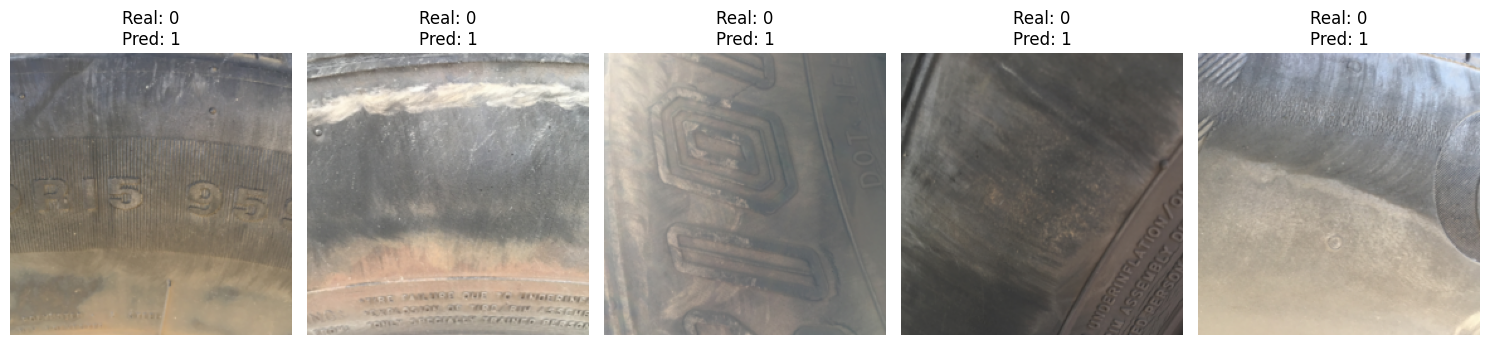
\includegraphics[width=0.9\textwidth]{Imagenes/analisis_fallos.png}
    \caption{Casos representativos de error del modelo ResNet-50 durante la validación (Etiqueta real vs Predicción).}
    \label{fig:fallos}
\end{figure}

\subsection{Conclusiones}
Este trabajo demuestra la viabilidad técnica de clasificar de forma automatizada texturas de neumáticos mediante arquitecturas convolucionales y aprendizaje por transferencia. Se concluye que:
\begin{itemize}
    \item El desbalance de datos debe ser mitigado mediante estrategias complementarias a nivel de datos (\texttt{WeightedRandomSampler}) y de pérdida (\texttt{Focal Loss}) para evitar que el gradiente ignore la clase minoritaria dañada.
    \item La transferencia de aprendizaje con ResNet-50 es significativamente superior (77.85\% exactitud y 0.8928 AUC-ROC en la versión con Focal Loss, y hasta 79.69\% de exactitud con la pérdida BCE) al entrenamiento desde cero de arquitecturas convolucionales simples, requiriendo además menor número de épocas de optimización.
    \item La interpretabilidad visual obtenida con Grad-CAM resulta indispensable para verificar que el clasificador enfoca su atención de forma justificada en los patrones texturales reales de desgaste y grietas físicas.
    \item Las limitaciones del sistema residen principalmente en la sensibilidad a variaciones externas de iluminación, desenfoque óptico y suciedad superficial, por lo que el despliegue comercial exige la estandarización de las cámaras y la limpieza de los neumáticos antes del escaneo.
\end{itemize}

% Análisis profundo de dónde falla el modelo y por qué, junto con las conclusiones.

% Referencias bibliográficas
\bibliographystyle{plainnat}
\begin{thebibliography}{5}
\providecommand{\natexlab}[1]{#1}
\providecommand{\url}[1]{\texttt{#1}}
\expandafter\ifx\csname urlstyle\endcsname\relax
  \providecommand{\doi}[1]{doi: #1}\else
  \providecommand{\doi}{doi: \begingroup \urlstyle{rm}\Url}\fi

\bibitem[He et al.(2016)He, Zhang, Ren, and Sun]{he2016deep}
Kaiming He, Xiangyu Zhang, Shaoqing Ren, and Jian Sun.
\newblock Deep residual learning for image recognition.
\newblock In \emph{Proceedings of the IEEE Conference on Computer Vision and Pattern Recognition}, pages 770--778, 2016.

\bibitem[Krizhevsky et al.(2012)Krizhevsky, Sutskever, and Hinton]{krizhevsky2012imagenet}
Alex Krizhevsky, Ilya Sutskever, and Geoffrey~E. Hinton.
\newblock Imagenet classification with deep convolutional neural networks.
\newblock In \emph{Advances in Neural Information Processing Systems}, volume~25, pages 1097--1105, 2012.

\bibitem[Lin et al.(2017)Lin, Goyal, Girshick, He, and Doll{\'a}r]{lin2017focal}
Tsung-Yi Lin, Priya Goyal, Ross Girshick, Kaiming He, and Piotr Doll{\'a}r.
\newblock Focal loss for dense object detection.
\newblock In \emph{Proceedings of the IEEE International Conference on Computer Vision}, pages 2980--2988, 2017.

\bibitem[Selvaraju et al.(2017)Selvaraju, Cogswell, Das, Vedantam, Parikh, and Batra]{selvaraju2017grad}
Ramprasaath~R. Selvaraju, Michael Cogswell, Abhishek Das, Ramakrishna Vedantam, Devi Parikh, and Dhruv Batra.
\newblock Grad-cam: Visual explanations from deep networks via gradient-based localization.
\newblock In \emph{Proceedings of the IEEE International Conference on Computer Vision}, pages 618--626, 2017.

\bibitem[Simonyan and Zisserman(2014)] {simonyan2014very}
Karen Simonyan and Andrew Zisserman.
\newblock Very deep convolutional networks for large-scale image recognition.
\newblock \emph{arXiv preprint arXiv:1409.1556}, 2014.

\end{thebibliography}

\end{document}
